% Template file for an a0 portrait poster.
% Written by Graeme, 2001-03 based on his SOC poster.
%
% See discussion and documentation at
% <http://www.astro.gla.ac.uk/users/norman/docs/posters/> 
%
%%%%%%%%%%%%%%%%%%%%%%%%%%%%%%%%%%%%%%%%
% Modified by Jozef Dobo\v{s} (c) 2011 % 
%%%%%%%%%%%%%%%%%%%%%%%%%%%%%%%%%%%%%%%%

\documentclass[a0,portrait]{a0poster}
% You might find the 'draft' option to a0 poster useful if you have
% lots of graphics, because they can take some time to process and
% display. (\documentclass[a0,draft]{a0poster})

\pagestyle{empty}
\setcounter{secnumdepth}{0}
\usepackage[absolute]{textpos}
\usepackage{txfonts}
\usepackage{wrapfig,times}
\usepackage{graphicx}
\usepackage{caption}
\usepackage{forloop}
\usepackage[margin=0cm]{geometry}
\usepackage{subfigure}
\usepackage{sidecap}
\usepackage{color}
\usepackage[colorlinks, pdfborder={0 0 0}]{hyperref}
\definecolor{LinkColor}{rgb}{0.75, 0, 0}
\definecolor{CiteColor}{rgb}{0, 0.5, 0.5}
\definecolor{UrlColor}{rgb}{0, 0, 0.75}
\hypersetup{linkcolor=LinkColor}
\hypersetup{citecolor=CiteColor}
\hypersetup{urlcolor=UrlColor}


%%%%%%%%%%
% Colors %
%%%%%%%%%%
\usepackage{color}
\definecolor{TitleColor}{rgb}{1,1,1} % white
\definecolor{BannerOneColor}{rgb}{0,0,0} % pitch black
\definecolor{BannerTwoColor}{rgb}{0.93,0.08,0.31} % pinky red
\definecolor{BannerThreeColor}{rgb}{0,0.27,0.48} % dark blue
\definecolor{BannerFourColor}{rgb}{0.33,0.19,0.098} % brown
\definecolor{BannerSixColor}{rgb}{0,0.27,0.42} % dark blue
\definecolor{BannerSevenColor}{rgb}{0.62,0.77,0.86} % sky blue
\definecolor{BannerEightColor}{rgb}{0.35,0.33,0.01} % military green
\definecolor{BannerNineColor}{rgb}{0.85,0.86,0.34} % lime green
\definecolor{BannerTenColor}{rgb}{0,0.66,0.80} % strong blue
\definecolor{BannerElevenColor}{rgb}{0.46,0,0.20} % maroon
\definecolor{BannerTwelveColor}{rgb}{0.37,0.32,0.44} % dark washed violet
\definecolor{BannerThirteenColor}{rgb}{0.79,0.84,0.65} % light washed green
\definecolor{BannerFourteenColor}{rgb}{0.57,0.64,0.27} % dark washed green
\definecolor{BannerFifteenColor}{rgb}{0.92,0.91,0.88} % unusable washed 
\definecolor{BannerSixteenColor}{rgb}{0.94,0.36,0.14} % strong orange
\definecolor{BannerSeventeenColor}{rgb}{0.97,0.61,0.19} % orange
\definecolor{BannerEighteenColor}{rgb}{0.99,0.76,0.11} % mustard yellow
\definecolor{BannerNineteenColor}{rgb}{0.79,0.76,0.73} % light gray-ish
\definecolor{BannerTwentyColor}{rgb}{0.63,0.58,0.54} % dark gray-ish

%%%%%%%%%%%%%%%%%%%%%%%%%%%%%%%%%%%%%%%%%%%%%%%%%%%%%%
% Only change here to affect all headings            %
\newcommand{\headingcolor}{\color{BannerSixColor}} 
%%%%%%%%%%%%%%%%%%%%%%%%%%%%%%%%%%%%%%%%%%%%%%%%%%%%%%

% see documentation for a0poster class for the size options here
%\let\Textsize\normalsize
\let\Textsize\Large
\def\Head#1{\noindent\hbox to \hsize{\hfil{\LARGE \headingcolor #1}}\bigskip}
\def\LHead#1{\noindent{\LARGE \bf \headingcolor \texttt{#1}}\smallskip}
\def\Authors#1{\noindent{\large #1}\smallskip}
\def\Subhead#1{\noindent{\large \headingcolor #1}}
\def\Title#1{\noindent{\Huge #1}}

% define the color of the emphasis text here. Please use a text color 
% consistent with the color scheme of the poster 
\def\emphasis#1{{\Large \color{BannerSeventeenColor} {#1}}}	


% Set up the grid
%
% Note that [0cm,0cm] is the margin round the edge of the page --
% it is _not_ the grid size. That is always defined as 
% PAGE_WIDTH/HGRID and PAGE_HEIGHT/VGRID. In this case we use
% 25 x 25. This gives us three wide columns for text (7 grid
% spacings) and four narrow columns (1 each) at each side of these 
% text columns
%
% Note however that texblocks can be positioned fractionally as well,
% so really any convenient grid size can be used.
%

% [margin, margin]{rows}{cols}
\TPGrid[0cm,0cm]{19}{25}  % 1 - 8 - 1 - 8 - 1 Columns

% Mess with these as you like
\parindent=0pt
%\parindent=1cm
\parskip=0.5\baselineskip
\linespread{1.1}

% abbreviations
\newcommand{\ddd}{\,\mathrm{d}}

\begin{document}

% Understanding textblocks is the key to being able to do a poster in
% LaTeX. In
%
%    \begin{textblock}{width}(x,y)
%    ...
%    \end{textblock}
%
% the first argument gives the block width in units of the grid
% cells specified above in \TPGrid; the second gives the (x,y)
% position on the grid, with the y axis pointing down.

%%%%%%%%%%%%%%
% Top Banner %
%%%%%%%%%%%%%%
% if you change this part, you can get matching color for headings
% in Colors section above
\begin{textblock}{20}(0,0)
%
\includegraphics[width=\paperwidth]{banners/banner11.pdf}

\includegraphics[height=3.7in]{banners/banner2.pdf}
\end{textblock}


%%%%%%%%%%%%%%%%%%%%%%%%%%%%%%%%%%%%%%%%%%%%%%%%%%%%%%%%%%%%%%%%%%%%%%%%%
%%%%%%%%%%%%%%%%%%%%%%%%%%%%%%%%%% Title %%%%%%%%%%%%%%%%%%%%%%%%%%%%%%%%
%%%%%%%%%%%%%%%%%%%%%%%%%%%%%%%%%%%%%%%%%%%%%%%%%%%%%%%%%%%%%%%%%%%%%%%%%
\begin{textblock}{17}(1,0.3)	 % syntax: {column_width} (x_coordinate, y_coordinate) in inches 
%\vspace*{-1cm}
{\color{TitleColor}
 \begin{center}
 { \Huge \bf{
 \noindent
 Event classification for a gravitational-wave inspiral search \\
 with a sine-Gaussian glitch veto \\
 \vspace*{-0.6cm}
 {\small LIGO Document G1500537} \par}
 }
 \end{center}
}
\end{textblock}

\begin{textblock}{15}(1,2.2)
\Authors{{\bf Shasvath J. Kapadia $^{*\dagger}$},~Thomas Dent$^\dagger$, ~Tito Dal Canton$^\dagger$} \\ 
\textit{$^*$ Department of Physics, University of Arkansas, Fayetteville, USA} \\
\textit{$^\dagger$ Albert-Einstein-Institut (Max-Planck-Institut f{\"ur} Gravitationsphysik), Hannover, Germany}\\

\end{textblock}

%%%%%%%%%%%%%%%%%%%%%% An example text block %%%%%%%%%%%%%%%%%%%%%%%%%%%%
%%%%%%%%%%%%%%%%%%%%%%%%%%%%%%%%%%%%%%%%%%%%%%%%%%%%%%%%%%%%%%%%%%%%%%%%%
\begin{textblock}{8}(1,3.4)
% syntax: {column_width} (x_coordinate, y_coordinate) in inches
% Please do not change the column_width and x_coordinate
  \LHead{Motivation}

\begin{itemize}
\item Gravitational waves (GWs) from inspiraling compact binaries -- neutron stars and black holes -- are 
likely first detections with advanced LIGO-Virgo.
\item Sensitivity of templated searches is limited by high signal-to-noise-ratio (SNR) events caused by non-Gaussian noise or ``glitches''.
\item To distinguish between glitches and real signals, recent searches used a $\chi^2$ test \cite{Allen2005} and ranked candidate events by ``re-weighted SNR'' $\hat{\rho}$ \cite{Babak}, a fixed function $\chi^2$ and SNR, both of which are properties of {\bf individual} events.
\item However some events with high $\hat{\rho}$ are still easily identified as glitches by examining surrounding data.
\item We propose using information from {\bf multiple} inspiral and sine-Gaussian triggers \cite{chatterji} {\bf around the time} of each candidate event to improve classification.
\end{itemize}
%Template based searches for inspiral GWs from neutron-star black hole (NS-BH) binaries requires separating high signal-to-noise ratio (SNR) events caused by GW signals from those induced by non-Gaussian noise or 'glitches'. Candidate events found in recent searches of LIGO-Virgo data were ranked via 'newSNR', a fixed function of the template matched filter SNR and chi-squared statistic, both of which are properties of each {\bf individual} candidate event. 
%
%We present here a multivariate classifier scheme, using features arising from {\bf multiple} inspiral and Omicron triggers around the time of the candidate event, where Omicron is a detector characterization pipeline that employs sine-Gaussian templates. 
\end{textblock}

\begin{textblock}{8}(1,7.7)
  \LHead{Inspiral Triggers}

\begin{itemize}
\item Triggers generated using non-spinning matched filter templates applied to simulated (glitchy) early aLIGO data injected with spinning inspiral signals.  Implementation and details of the simulations are described in \cite{Tito}.
%\item As seen in Figure \ref{fig:InspiralTrigs}, it becomes straightforward to distinguish between signal and noise events by looking at triggers within a time window centred on the candidate events. 
\end{itemize}

\begin{figure}
%\centering
\hspace{-1cm}
%\subfigure[]
{
  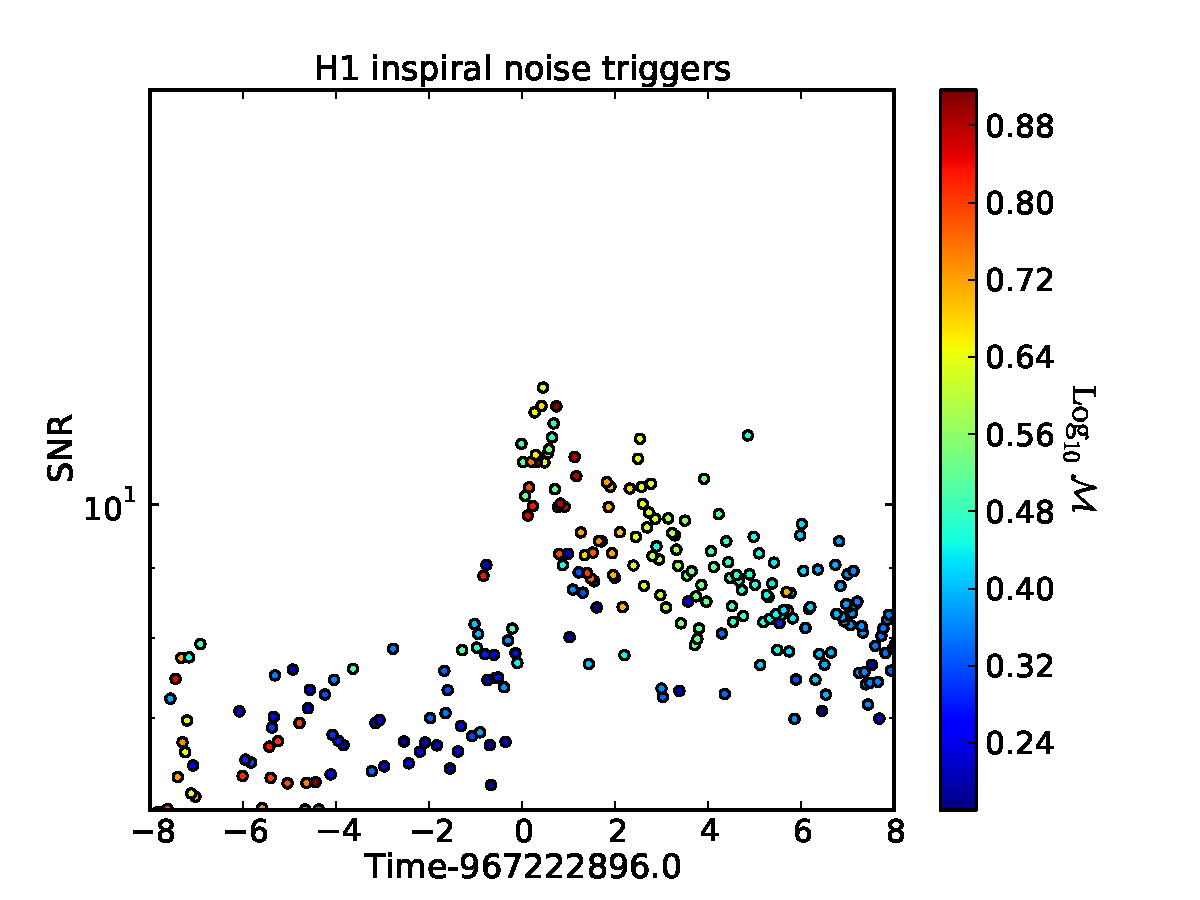
\includegraphics[scale=0.96]{images/H1-inspiral-noise-trigs_POSTER.pdf}
  }
\hspace{-2cm}
%\subfigure[]
{
  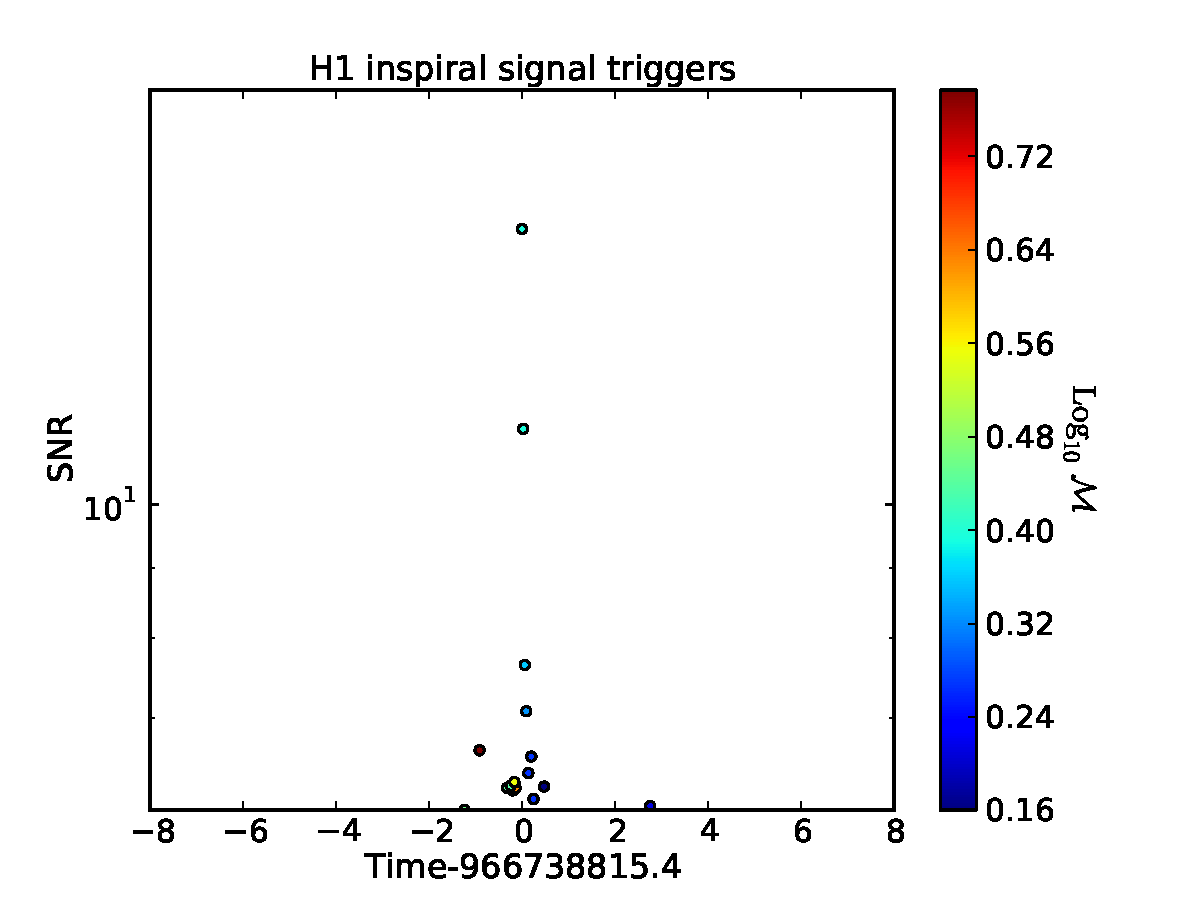
\includegraphics[scale=0.96]{images/H1-inspiral-signal-trigs_POSTER.pdf}
  }
\vspace*{-1cm}
\caption{Inspiral triggers around a high-$\hat{\rho}$ noise event (left) and simulated signal event (right). %\\
Excess triggers produced over a time window in glitchy data are clearly distinguishable from the `clean' signal.
}

\label{fig:InspiralTrigs}
\end{figure}

\end{textblock}

\begin{textblock}{8}(1,13.7)
  \LHead{Omicron Triggers}

\begin{itemize}
\item Triggers generated using sine-Gaussian templates and ``clustered'' together into tiles if occuring within a short enough time interval.
\item For simulated inspiral signals, high-SNR tiles fall along the Newtonian inspiral time-frequency track; for noise events, the tiles' time and frequency have more random scatter -- see Figure \ref{fig:OmicronTrigs}.
\item Information provided by Omicron triggers can contribute to more accurate classification of candidate inspiral events.
\end{itemize}
  
\begin{figure}
%\centering
%\subfigure[]
\hspace{-1cm}
{
  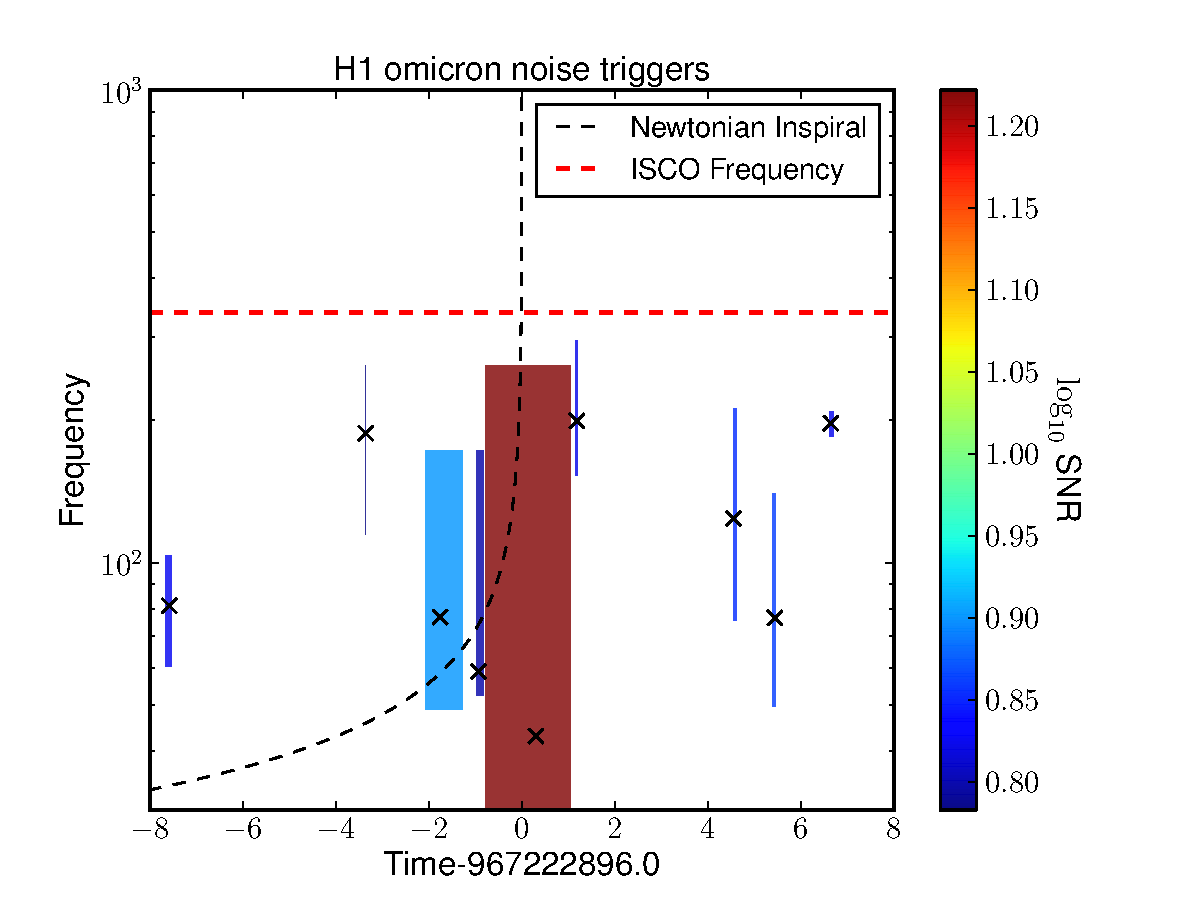
\includegraphics[scale=0.96]{images/H1-omicron-noise-trigs_POSTER.pdf}
  }
\hspace{-2cm}
%\subfigure[]
{
  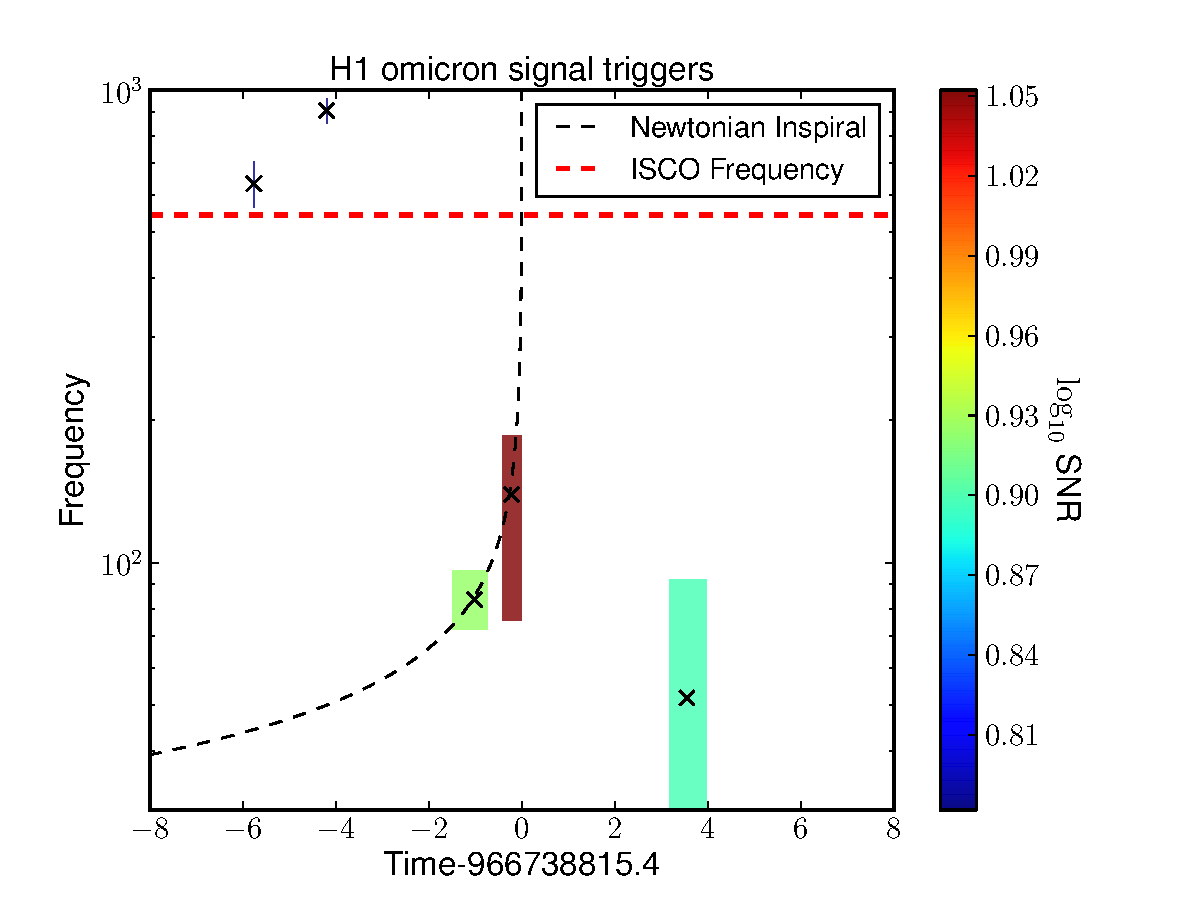
\includegraphics[scale=0.96]{images/H1-omicron-signal-trigs_POSTER.pdf}
  }
\vspace*{-1cm}
\caption{Clustered Omicron triggers (tiles) around the same noise (left) and signal (right) events as in Figure~\ref{fig:InspiralTrigs}. 
The dimensions of each rectangle give the duration and bandwidth of the clustered tile. The x-mark shows the frequency and time of the loudest trigger in each cluster.}
\label{fig:OmicronTrigs}
\end{figure}

\end{textblock}

\begin{textblock}{8}(1,21.2)
  \LHead{Classification Features}

Features are constructed from individual events and their neighbouring triggers, that could help discriminate between signals and glitches:
\begin{itemize}
\item Inspiral SNR and chirp mass of candidate event
\item Number of nearby inspiral and Omicron triggers
\item Individual properties of loudest nearby inspiral and Omicron triggers
\item Time lag between loudest nearby Omicron trigger and Newtonian inspiral track
\end{itemize}
\end{textblock}


\begin{textblock}{8}(10,3.4)
  \LHead{The Random Forest (RF) Classifier}

\begin{SCfigure}\label{fig:RF}
%\centering
\hspace{-3cm}
%\vspace{-1cm}
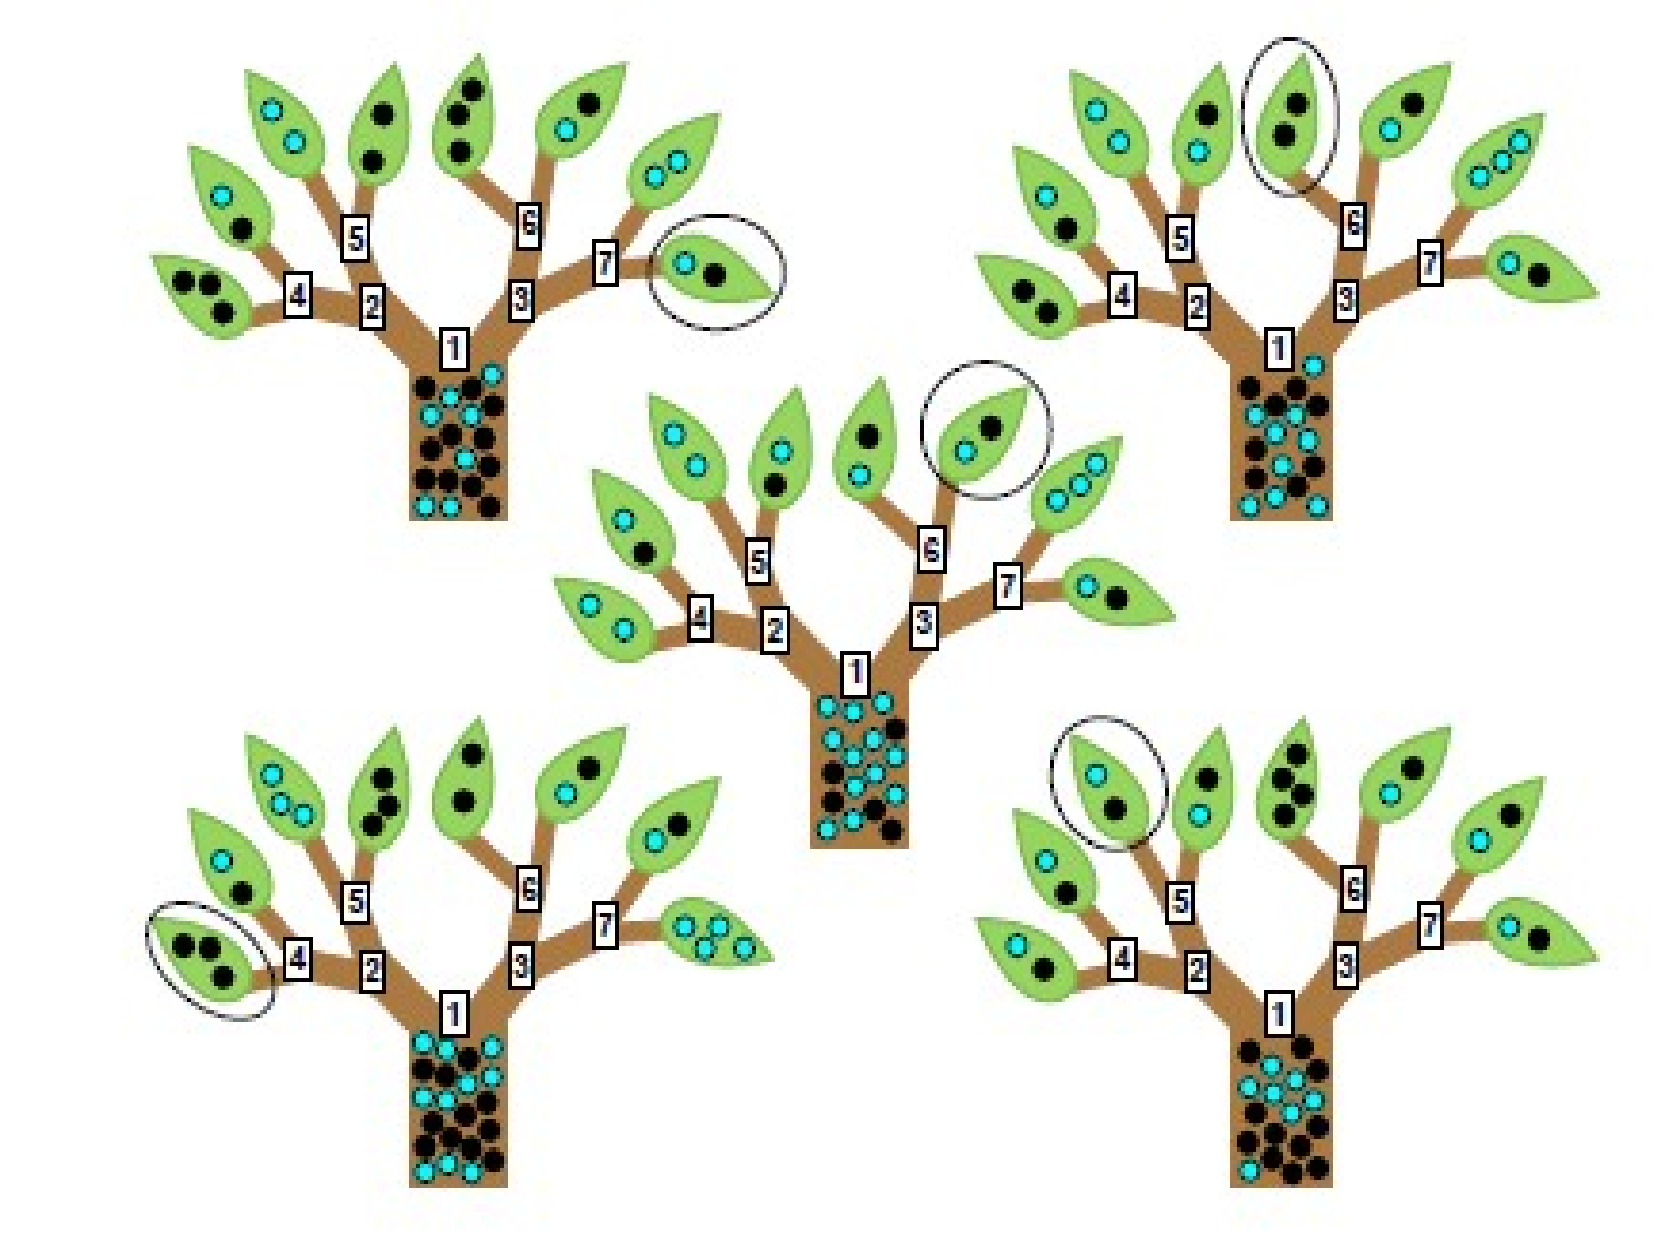
\includegraphics[scale=0.7]{images/RandomForest.pdf}
\caption{The RF contains many decision trees, each trained on a randomized subset of noise and signal events. An event given to the RF for classification goes from root node to leaf node on each tree, following a path determined by the splitting condition imposed at each node. The RF assigns a ranking score to the event by computing the distribution of training events, in the leaves where the event is placed, over all trees. Picture taken from \cite{MVSC}.}
\end{SCfigure}
\end{textblock}

\begin{textblock}{8}(10,8.0)
  \LHead{Results: Varying RF parameters}
\begin{itemize}
\item We use a 2-fold `round robin': splitting the data into two parts, training the RF on one part and evaluating scores for the other.
\item Assign false alarm probability (FAP) values to simulated signals by comparing their scores to noise events and compute a weighted sum over simulated signals as a measure of the expected number of detections. 
%\item Evaluate performance of the classifier on our data set by a weighted sum over simulated signals, proportional to expected number of detections
\item Errors estimated over 5 realizations of random 2-fold splitting.
\end{itemize}

\begin{figure}\label{ROC_Plots_RF}
%\centering
%\subfigure[]
%{
%  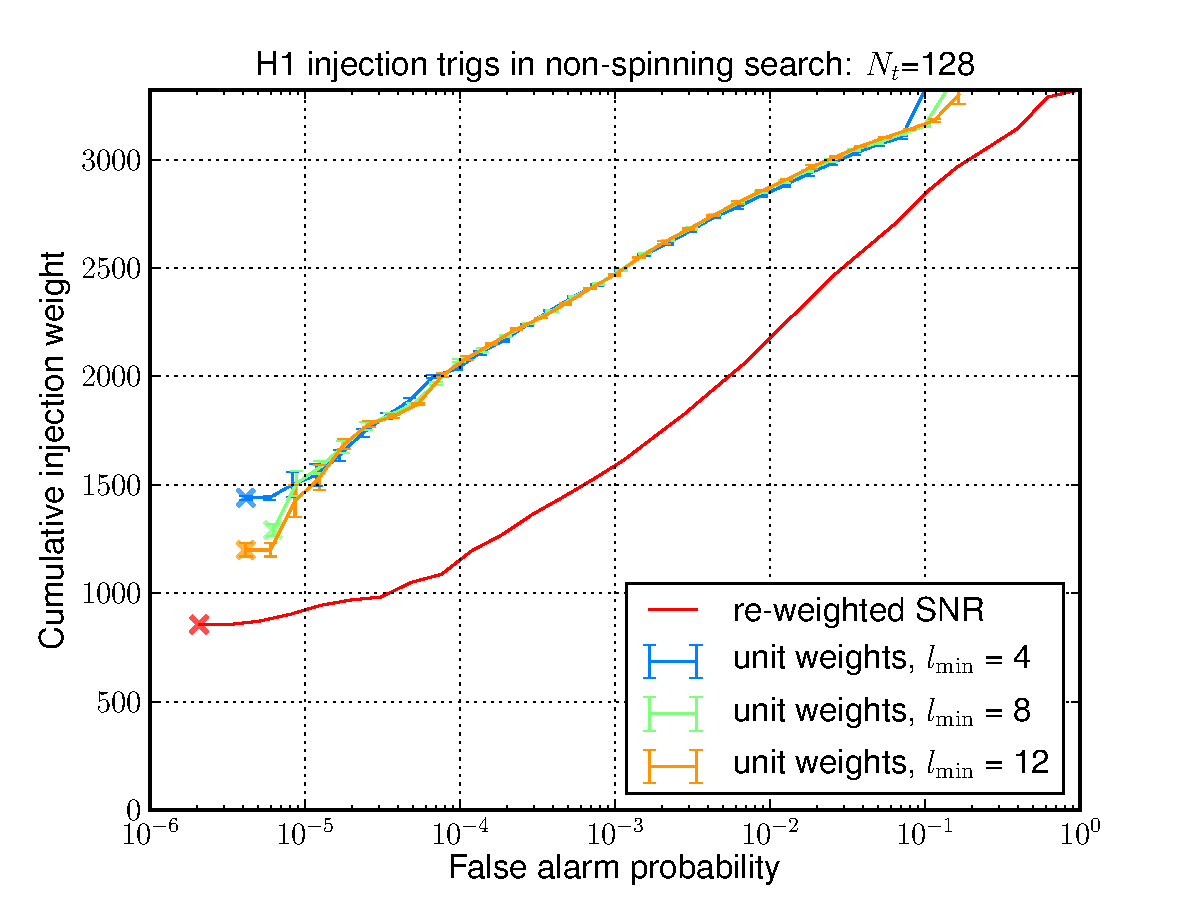
\includegraphics[scale=0.8]{images/H1-merged_nospin_ROC_t128_w1_l4-8-12_POSTER.pdf}
%  }
%\hspace{-3.5cm}
%\subfigure[]
{
  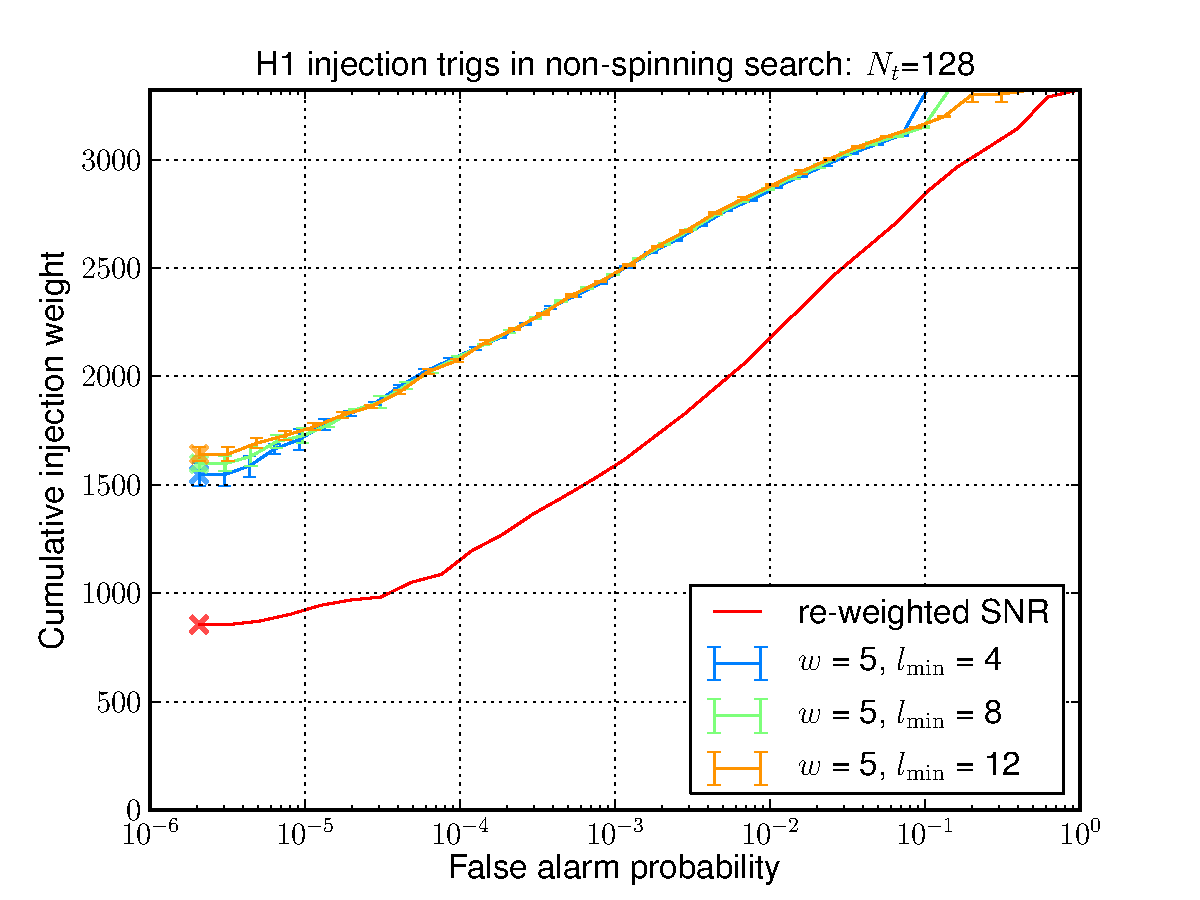
\includegraphics[scale=0.88]{images/H1-merged_nospin_ROC_t128_w5_l4-8-12_POSTER.pdf}
  }
%\subfigure[]
%\hspace{-1cm}
%{
%  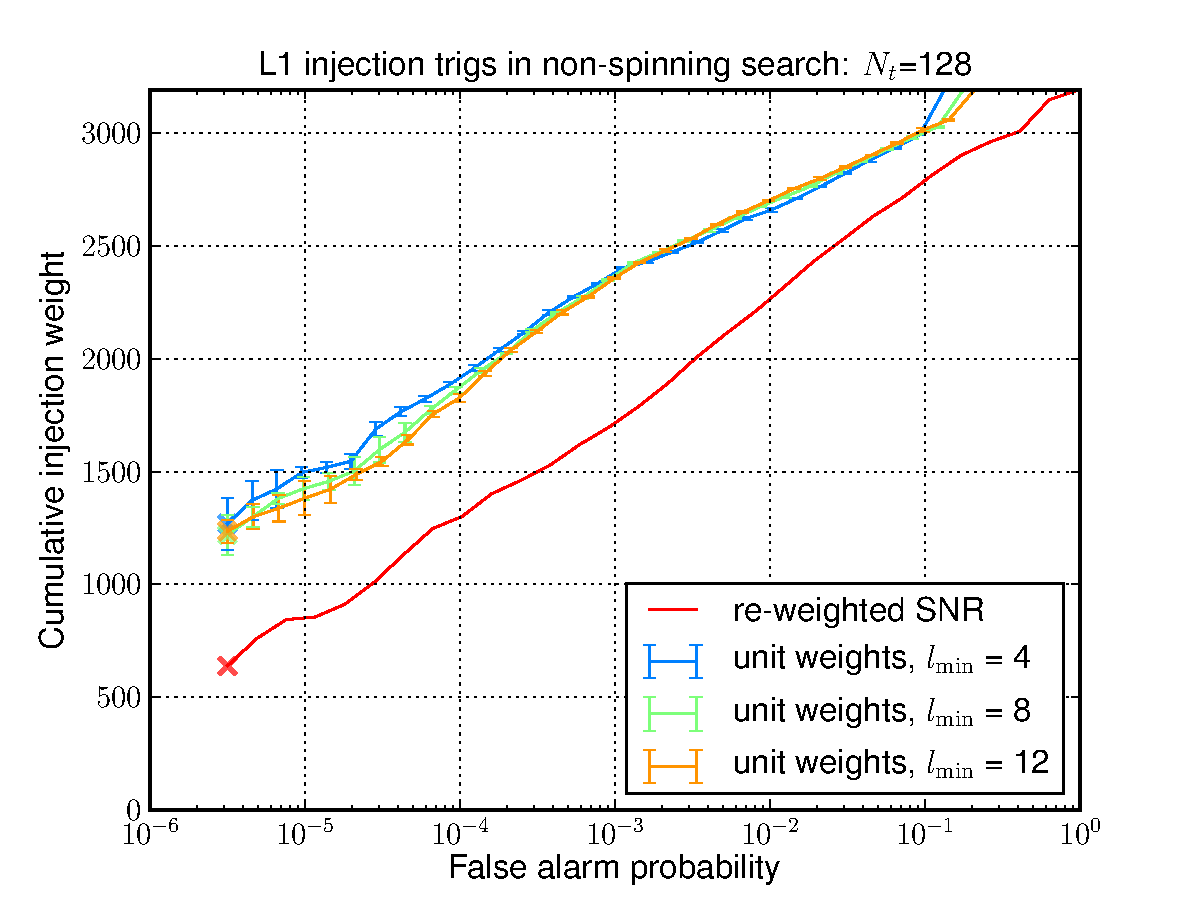
\includegraphics[scale=0.88]{images/L1-merged_nospin_ROC_t128_w1_l4-8-12_POSTER.pdf}
%  }
\hspace{-1cm}
%\subfigure[]
{
  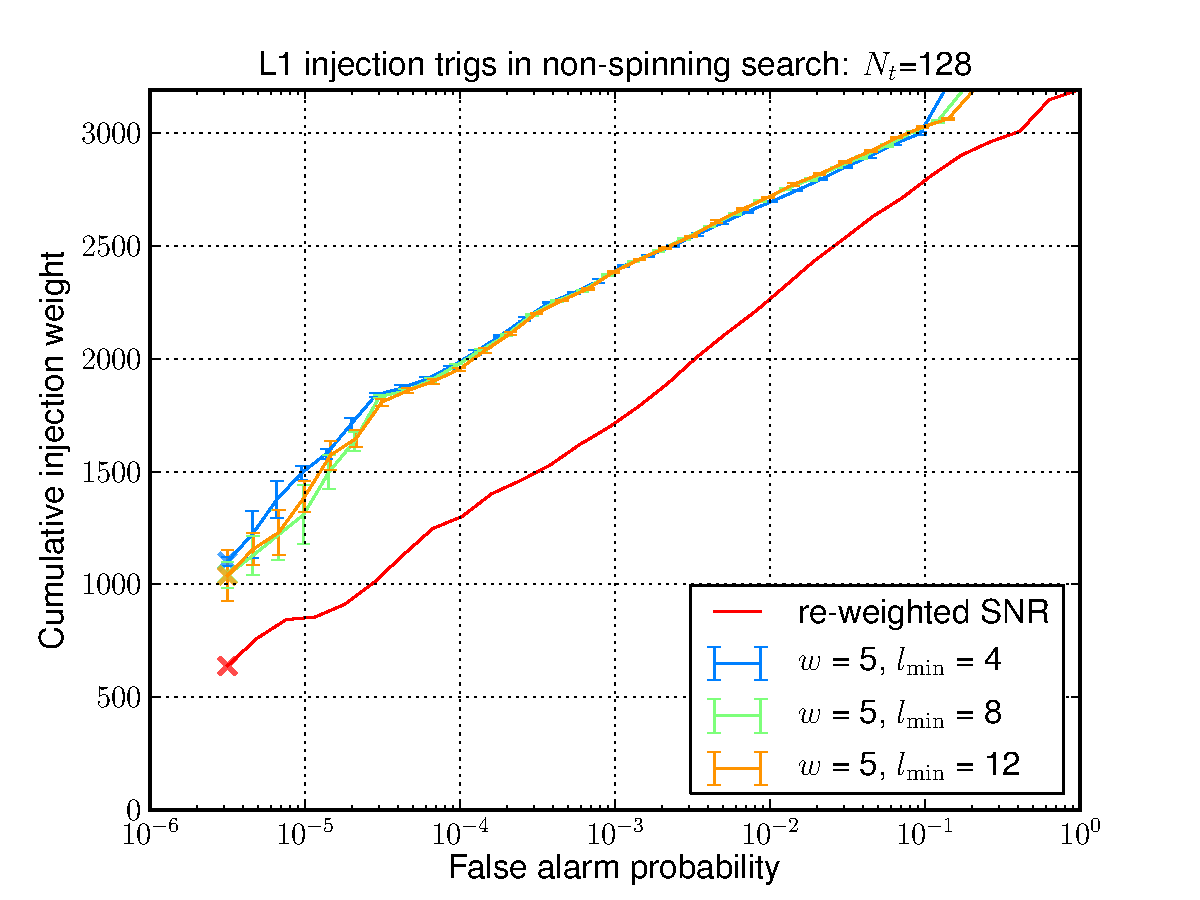
\includegraphics[scale=0.88]{images/L1-merged_nospin_ROC_t128_w5_l4-8-12_POSTER.pdf}
  }
\hspace{-2cm}
\vspace*{-1cm}
\caption{Performance of the classifier for different RF parameters and for data sets from different detectors.  The classifier is able to detect a consistently higher number of simulated signals above noise, as compared to ranking by re-weighted SNR.}
\end{figure}

\end{textblock}

\begin{textblock}{8}(10,15.0)
  \LHead{Results: Adding $\chi^2$ as a feature}
%\begin{itemize}
%We also investigated whether the classifier's performance could be improved by using the event's $\chi^2$ value as an additional feature :
%\end{itemize}
\begin{figure}\label{fig:ROC_Plots_chisq}
%\centering
{
  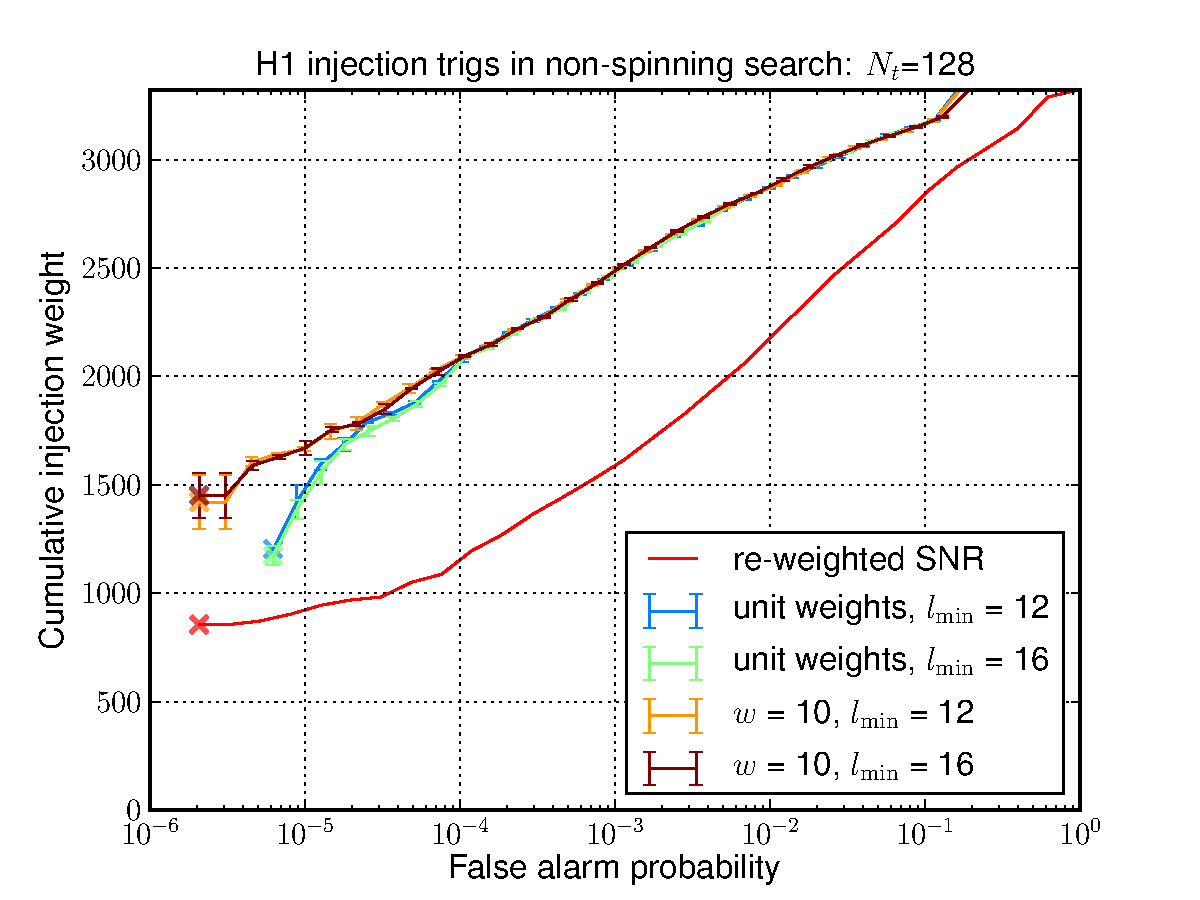
\includegraphics[scale=0.88]{images/H1-merged_nospin_ROC_chisq_t128_w1-10_l12-16_POSTER.pdf}
}
\hspace{-1cm}
{
  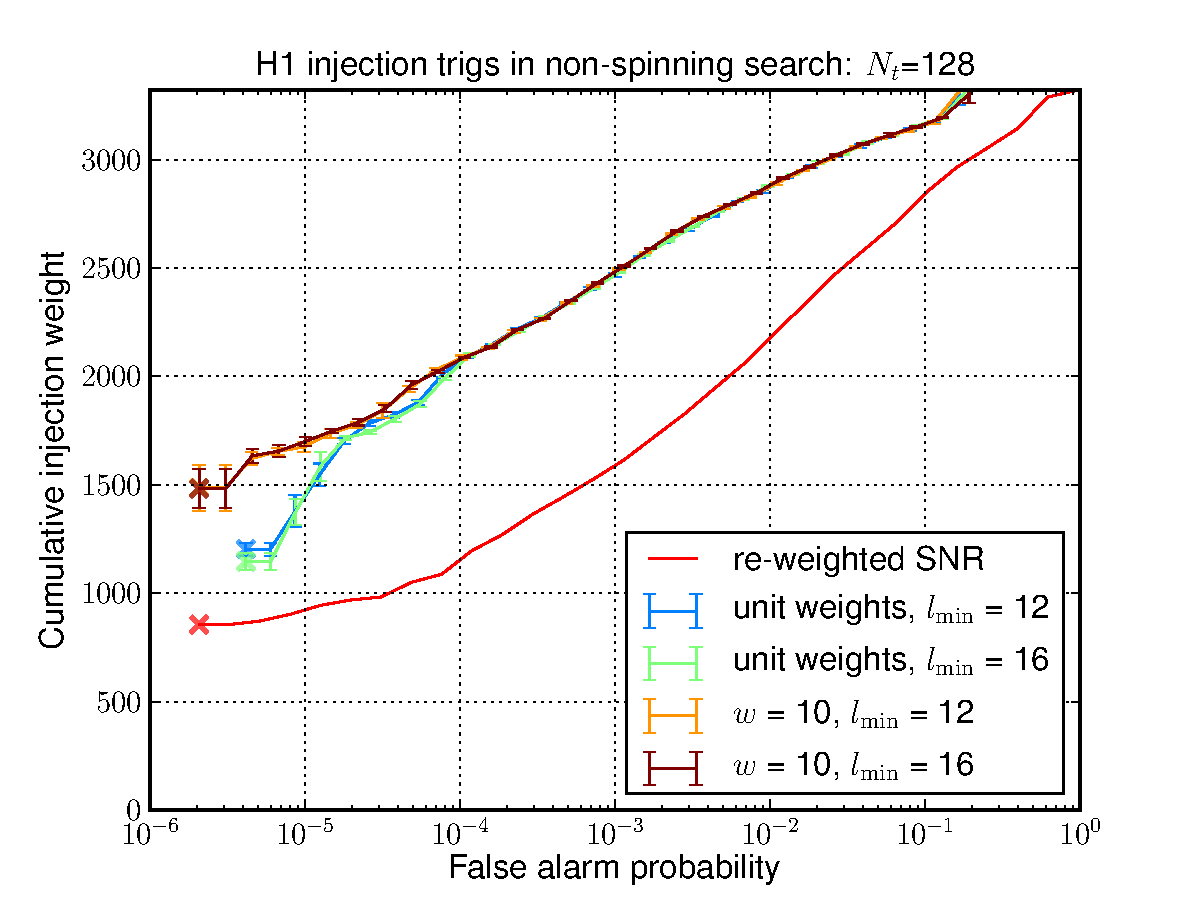
\includegraphics[scale=0.88]{images/H1-merged_nospin_ROC_t128_w1-10_l12-16_POSTER.pdf}
}
\hspace{-2cm}
\vspace*{-2cm}
\caption{With (left) and without (right) $\chi^2$: Adding $\chi^2$ values to the classifier does not yield further increases in the expected number of detections.}
\end{figure}

%\end{itemize}

 
\end{textblock}

\begin{textblock}{8}(10,19.25)
  \LHead{Summary and Outlook}

\begin{itemize}
\item Using a multivariate classifier based on features from multiple inspiral and sine-Gaussian triggers around candidate events, we find an almost 2-fold increase in the expected number of inspiral signals recovered at low FAP, in glitchy data, as compared to ranking via re-weighted SNR. 
\item Features we have identified are able to substitute for and improve on the $\chi^2$ test, for spinning signals recovered with non-spinning templates.
\item Currently the classifier is implemented for single-detector clustered inspiral triggers; more development is required to extend it to a multi-detector analysis.
\end{itemize}
  

%%%%%%%%%%%%%%%%%%%%%%%%%%%%%%%%%%%%%%%%%%%%%%%%%%%%%%%%%%%%%%%%%%%%%%%%%
%%%% You shouldn't need to touch this unless you want to remove the %%%%%
%%%%%%%%%%%%%%%%%%%%%%%%% entire reference section %%%%%%%%%%%%%%%%%%%%%%
\vspace{0.5cm}
\Subhead{References}
\begin{small}
\begingroup
\renewcommand{\section}[2]{}%
\begin{thebibliography}{99}
%%%%%%%%%%%%%%%%%%%%%%%%%%%%%%%%%%%%%%%%%%%%%%%%%%%%%%%%%%%%%%%%%%%%%%%%%%
%
%%%%%%%%%%%%%%%%%%%%%%%%%%%%%%%%%%%%%%%%%%%%%%%%%%%%%%%%%%%%%%%%%%%%%%%%%%
%%%%%%%%%%%%%%%%%%%%%%%%%%% Add your references here %%%%%%%%%%%%%%%%%%%%%
%%%%%%%%%%%%%%%%%%%%%%%%%%%%%%%%%%%%%%%%%%%%%%%%%%%%%%%%%%%%%%%%%%%%%%%%%
\bibitem{Allen2005} B. Allen, Phys. Rev. D {\bf 71}, 062001 (2005) 
\bibitem{Babak} S. Babak {\it et al}, Phys. Rev. D {\bf 87}, 024033, (2012)
\bibitem{chatterji} S. Chatterji, Ph.D. thesis, Massachussetts Institute of Technology, (1995)
\bibitem{Tito} T. Dal Canton {\it et al}, Phys. Rev. D {\bf 90}, 082004, (2014) 
\bibitem{MVSC} P. T. Baker {\it et al}, Phys. Rev. D {\bf 91}, 062004, (2015) 
%%%%%%%%%%%%%%%%%%%%%%%%%%%%%%%%%%%%%%%%%%%%%%%%%%%%%%%%%%%%%%%%%%%%%%%%%

\end{thebibliography}
\end{small}
\endgroup
\end{textblock}


%%%%%%%%%%%%%%%%%%%%%%%%%%%%%%%%%%%%%%%%%%%%%%%%%%%%%%%%%%%%%%%%%%%%%%%%%
%%%%%%%%%%%%%% Place the institute logos at the bottom left %%%%%%%%%%%%
%%%%%%%%%%%%%%%%%%%%%%%%%%%%%%%%%%%%%%%%%%%%%%%%%%%%%%%%%%%%%%%%%%%%%%%%%
\begin{textblock}{18}(13.7,2.2)    
\resizebox{1.7\TPHorizModule}{!}{
\includegraphics{images/UA_Logo_Horizontal.png}} \hspace{2cm}
\resizebox{0.5\TPHorizModule}{!}{
\includegraphics{images/LogoAEI.png}} \hspace{2cm}
\resizebox{0.8\TPHorizModule}{!}{
\includegraphics{images/LogoMinerva.jpg}}
\end{textblock}

\begin{textblock}{18}(16.5,0.17)    
\resizebox{2.3\TPHorizModule}{!}{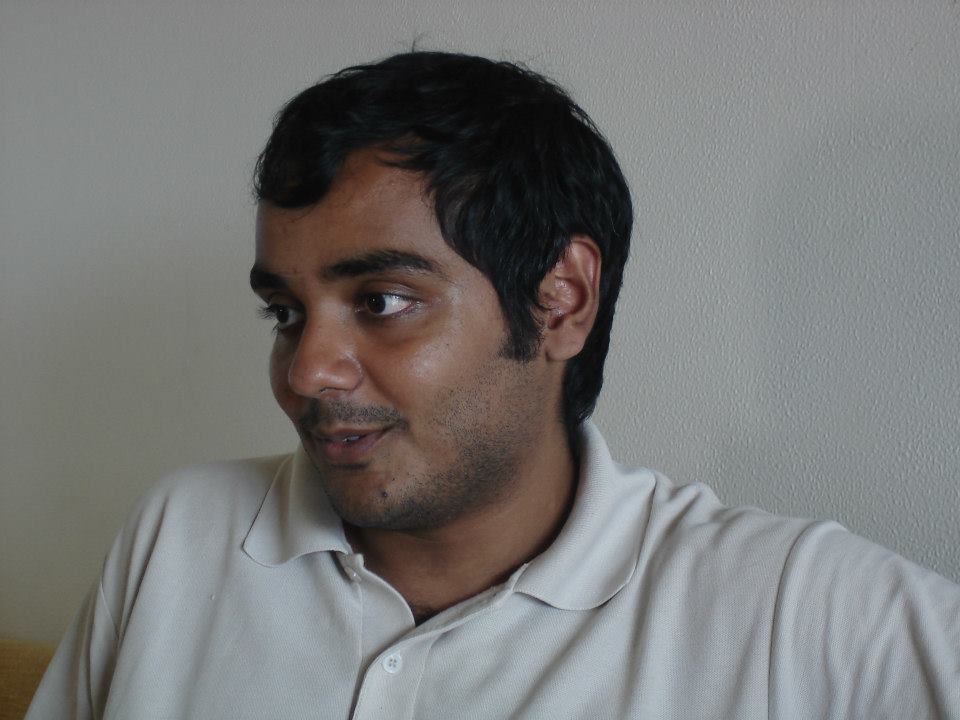
\includegraphics{images/shasvath_photo.jpg}} 
\end{textblock}
%%%%%%%%%%%%%%%%%%%%%%%%%%%%%%%%%%%%%%%%%%%%%%%%%%%%%%%%%%%%%%%%%%%%%%%%%

%%%%%%%%%%%%%%%%%%%%%%%%%%%%%%%%%%%%%%%%%%%%%%%%%%%%%%%%%%%%%%%%%%%%%%%%%
%%%%%%%%%%%%%%%%%%%%%%%%%%%% Acknowledgments %%%%%%%%%%%%%%%%%%%%%%%%%%%%
%%%%%%%%%%%%%%%%%%%%%%%%%%%%%%%%%%%%%%%%%%%%%%%%%%%%%%%%%%%%%%%%%%%%%%%%%
%\begin{textblock}{7}(9,23.2)
%\Subhead{Acknowledgments}
%\small{We thank so and so for this and that ... Lorem ipsum dolor sit amet, consectetur adipiscing elit. Phasellus dignissim auctor semper. In vitae risus eu lacus varius blandit quis vel quam. Vestibulum hendrerit ligula lacus, non lacinia mi}
%\end{textlock}
%%%%%%%%%%%%%%%%%%%%%%%%%%%%%%%%%%%%%%%%%%%%%%%%%%%%%%%%%%%%%%%%%%%%%%%%%

\end{document}

